\documentclass[conference]{IEEEtran}
\IEEEoverridecommandlockouts
% The preceding line is only needed to identify funding in the first footnote. If that is unneeded, please comment it out.
\usepackage{amsmath,amssymb,amsfonts}
\usepackage{algorithmic}
\usepackage{graphicx}
\usepackage{textcomp}
\usepackage{xcolor}
\usepackage{enumitem}
\def\BibTeX{{\rm B\kern-.05em{\sc i\kern-.025em b}\kern-.08em
    T\kern-.1667em\lower.7ex\hbox{E}\kern-.125emX}}

\makeatletter % changes the catcode of @ to 11
\newcommand{\linebreakand}{%
  \end{@IEEEauthorhalign}
  \hfill\mbox{}\par
  \mbox{}\hfill\begin{@IEEEauthorhalign}
}
\makeatother % changes the catcode of @ back to 12

\usepackage{booktabs}
\usepackage{multirow}
\usepackage[labelfont=bf,textfont=it]{caption}
\usepackage{subcaption}
\usepackage[sort&compress,numbers]{natbib}
\usepackage{listings}

\usepackage{hyperref}
\hypersetup{
    colorlinks,
    linkcolor={blue},
    citecolor={blue},
    urlcolor={blue},
    breaklinks=true,
    plainpages=true
}

\newcommand{\cref}[3]{\hyperref[#2]{#1~\ref*{#2}{#3}}}
% Color references
\newcommand{\colref}[2]{\hyperref[#2]{#1~\ref*{#2}}}
\newcommand{\eqnref}[1]{\colref{Eq.}{#1}}
\newcommand{\figref}[1]{\colref{Fig.}{#1}}
\newcommand{\subfigref}[2]{\cref{Figure}{#1}{#2}}
\newcommand{\figsref}[2]{\crefs{Figures}{#1}{#2}}
\newcommand{\secref}[1]{\colref{Section}{#1}}
\newcommand{\appref}[1]{\colref{}{#1}}
\newcommand{\tabref}[1]{\colref{Table}{#1}}
\newcommand{\algref}[1]{\colref{Algorithm}{#1}}
\newcommand{\defref}[1]{\colref{Definition}{#1}}
\newcommand{\Algref}[1]{\colref{Algorithm}{#1}}



\lstset{
basicstyle=\ttfamily\scriptsize, breaklines=true, frame=single, numbers=left, numberstyle=\tiny, columns=flexible, }

\begin{document}

% \title{CRAFT: A Multi-Agent Pipeline for Zero-Shot\\Text-to-Parametric CAD Generation}
\title{CRAFT: Corrective and Robust Multi-Agent Framework for Text-to-Parametric CAD\\
% \thanks{a. Iowa State University, USA}
% \thanks{b. New York University, USA}
% \thanks{This work was supported by the National Science Foundation under grant CMMI-AM-2347623/2347624. We would like to thank the NVIDIA Corporation for providing GPUs for academic research.}
}

% Double-blind: no author info

\author{\IEEEauthorblockN{Anonymous Authors}
\IEEEauthorblockA{Anonymous Institution}}

% % Musthafa, Anushrut, Mehdi, Chinmay, Aditya, Adarsh
% \author{\IEEEauthorblockN{Mohammad Musthafa Rafi\textsuperscript{a} 
% \and Anushrut Jignasu\textsuperscript{a}
% \and Mehdi Saraeian\textsuperscript{a}
% \and Chinmay Hegde\textsuperscript{b}
% \and Aditya Balu\textsuperscript{a}
% \linebreakand
% Adarsh Krishnamurthy\textsuperscript{a}}
% \IEEEauthorblockA{Email: \textsuperscript{a} (musthafa | anushrutg | mehdis | baditya | adarsh)@iastate.edu , \textsuperscript{b} chinmay.h@nyu.edu}
% }

\maketitle

\begin{abstract}
Text-to-CAD generation has the potential to make mechanical CAD more accessible, but existing approaches face a trade-off between data dependence and output fidelity. Supervised methods rely on large paired text--model datasets, while zero-shot prompting strategies are often brittle and tend to lose the parametric structure needed for downstream editing and customization. We present CRAFT, a corrective and robust multi-agent framework that produces parametric OpenSCAD programs from natural language without task-specific training. At its core is a JSON intermediate representation that preserves symbolic parametric expressions throughout the generation process, enabling models to remain editable rather than collapsing into hard-coded geometry. CRAFT combines semantic understanding, parametric planning, compilation, rendering, self-correction, and component-level verification within a layered recovery process, using multi-view visual feedback to detect and repair geometric errors. Our results show that structured corrective generation produces reliable and customizable CAD models that are competitive with more heavily supervised alternatives.
\end{abstract}

\begin{IEEEkeywords}
Text-to-CAD, parametric modeling, multi-agent systems, large language models, zero-shot generation, OpenSCAD
\end{IEEEkeywords}






\section{Introduction}
\label{Sec:intro}

Text-driven geometric modeling has seen rapid progress in recent years, with large language and vision models enabling increasingly capable systems for generating 3D shapes directly from natural language descriptions~\citep{zhang2026llmcad,poole2023dreamfusion,jun2023shape,nichol2022pointe}. These advances have raised the prospect of making mechanical computer-aided design (CAD) accessible to users without specialized CAD expertise, reducing the barrier between a design intent expressed in words and a manufacturable geometric model. Despite this progress, existing approaches remain brittle in practice. Supervised methods that fine-tune models on paired text--CAD datasets can produce geometrically plausible outputs within their training distribution, but generalize poorly to novel shapes and require substantial curated data to train~\citep{text2cad2024,cadcoder2025,text2cadquery2025,li2025llm4cad}. Zero-shot prompting strategies avoid this data dependency but are prone to generating syntactically invalid code, non-renderable geometry, and outputs that fail to faithfully reflect the original prompt. Critically, both families of approaches tend to produce hard-coded numeric geometry rather than editable parametric models, limiting their utility for downstream engineering and customization tasks~\citep{wu2021deepcad,fusion360gallery2021}.

Agentic systems offer a natural path toward addressing these limitations~\citep{guo2024multiagent,madaan2023selfrefine}. Rather than treating CAD generation as a single forward pass, a multi-agent pipeline can decompose the problem into discrete stages, including semantic understanding, structured planning, code synthesis, and verification, each of which can be independently validated and repaired. This staged architecture allows errors to be detected and corrected locally rather than propagating silently into the final output, improving both reliability and geometric fidelity. A particularly well-suited target for such a pipeline is OpenSCAD~\citep{openscad}, a declarative scripting language in which geometry is expressed as a program over symbolic parameters. Generating OpenSCAD code rather than mesh geometry preserves the parametric relationships that make CAD models editable and reusable. However, verifying the correctness of generated OpenSCAD programs is non-trivial: a program may compile successfully yet produce geometry that is visually or dimensionally incorrect relative to the prompt. Effective verification, therefore, requires grounding generated outputs in external reference knowledge, both to check that recognized components conform to standard specifications and to confirm that expected parts are geometrically present. NopSCADlib~\citep{nopscadlib} is a parametric OpenSCAD component library that provides catalog-defined specifications for standard mechanical parts. These specifications ground generated outputs in physically meaningful dimensions and enable verification of component completeness.

\begin{figure*}[t!]
    \centering
    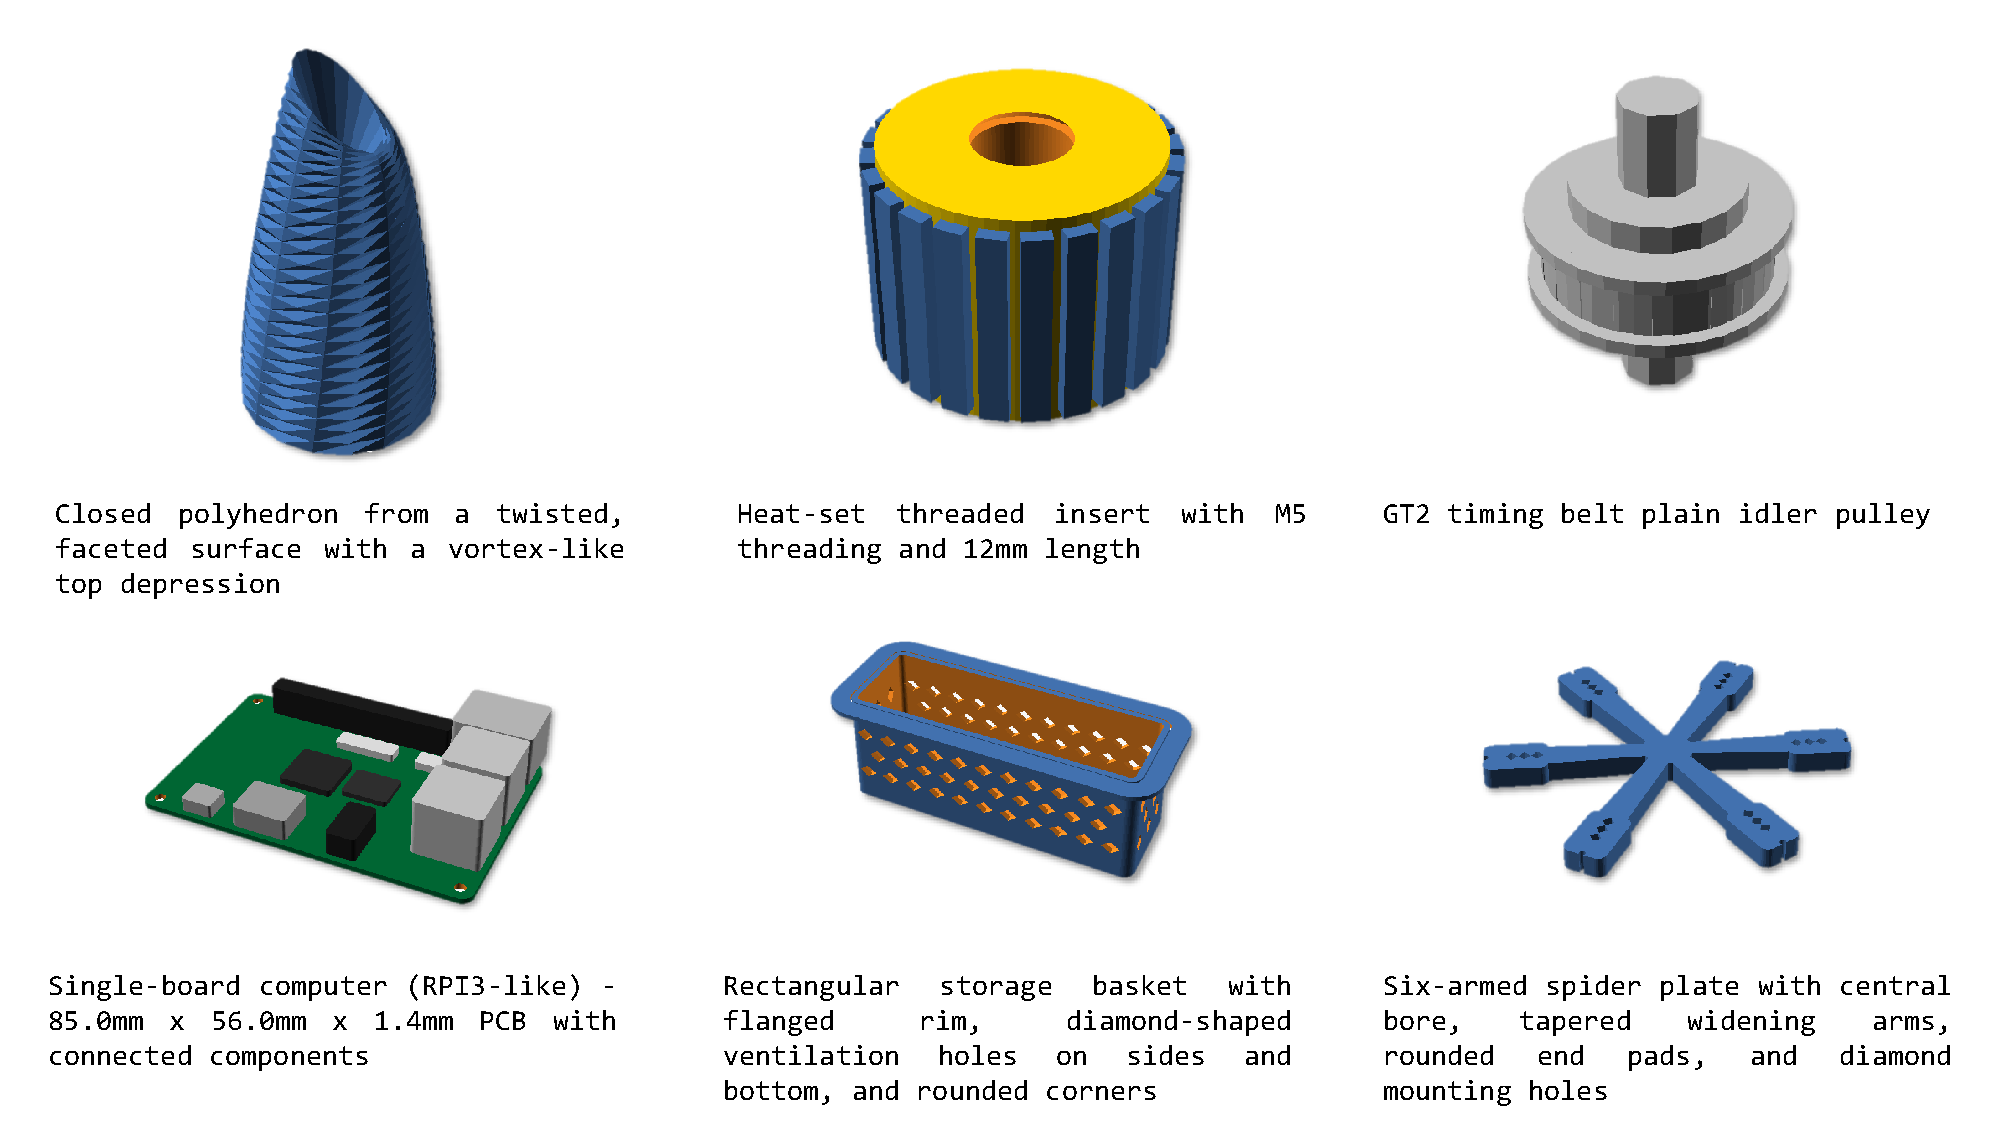
\includegraphics[width=0.85\linewidth]{figures/pdf/CRAFT_Examples.pdf}
    \caption{Examples of different CAD models created by CRAFT from the prompts.}
    \label{Fig:teaser}
\end{figure*}


We present CRAFT (\figref{Fig:teaser}), a corrective and robust multi-agent framework for text-to-parametric CAD generation. CRAFT produces executable and editable OpenSCAD programs from natural language without task-specific training through three core mechanisms: a JSON-based intermediate representation that preserves symbolic parametric expressions, multi-view visual feedback to detect and correct geometric errors, and a layered recovery strategy to handle failures at every stage of the pipeline. Our main contributions are as follows:
\begin{itemize}[topsep=0pt]
\item We develop a corrective and robust six-stage multi-agent framework for zero-shot text-to-parametric CAD generation that combines structured planning, multi-view visual verification, and layered error recovery to produce executable OpenSCAD programs from natural language.
\item We propose a JSON-based intermediate representation that preserves symbolic parametric expressions throughout the generation process, enabling the produced CAD programs to remain editable and reusable rather than collapsing into hard-coded geometry.
\item We evaluate CRAFT across three datasets (NopSCADlib, ABC, and Slice-100K) and show that it achieves competitive perceptual and geometric quality relative to direct generation baselines.
\end{itemize}

% The rest of the paper is arranged as follows: we provide a brief overview of related work in \secref{Sec:related}; the proposed CRAFT framework and its components are described in \secref{Sec:method}; experimental setup, datasets, and evaluation metrics are detailed in \secref{Sec:setup}; quantitative and qualitative results are presented and analyzed in \secref{Sec:results}; \secref{Sec:discussion} discusses the broader implications, limitations, and directions for future work; and \secref{Sec:conclusion} concludes the paper.

\section{Related Work}
\label{Sec:related}

\textbf{Text-to-3D and Text-to-CAD Generation.} Generative approaches to 3D modeling have advanced rapidly, spanning neural implicit representations~\citep{poole2023dreamfusion}, point cloud synthesis~\citep{nichol2022pointe}, and shape generation from text~\citep{jun2023shape}. While these methods produce visually compelling outputs, they typically yield fixed mesh geometry that cannot be edited parametrically or reused in engineering workflows. A parallel line of work targets CAD-specific representations. Text2CAD~\citep{text2cad2024} generates sequential CAD construction sequences from natural language, while LLM4CAD~\citep{li2025llm4cad} explores multimodal models for 3D CAD generation. CAD-Coder~\citep{cadcoder2025} fine-tunes a language model on text--CadQuery pairs with reinforcement learning using geometric rewards, and Text-to-CadQuery~\citep{text2cadquery2025} scales this paradigm through larger paired datasets. These supervised approaches achieve strong in-distribution results but require curated paired training data and produce outputs that are often not directly editable as parametric programs. CRAFT avoids task-specific training entirely and instead uses structured zero-shot generation to produce symbolic, editable OpenSCAD programs.

\textbf{Program Synthesis and Code Generation.} Generating executable code from natural language has become a well-studied problem, with large language models demonstrating strong performance across programming tasks~\citep{chen2021codex}. Techniques such as chain-of-thought prompting~\citep{wei2022chainofthought} and self-refinement~\citep{madaan2023selfrefine} have shown that decomposing generation into reasoning steps improves correctness on structured outputs. These ideas are particularly relevant for CAD, where generated programs must satisfy multiple simultaneous constraints: syntactic validity, successful compilation, geometric correctness, and semantic alignment with the input prompt. Direct single-shot generation is often insufficient in this setting, motivating the use of intermediate representations and iterative repair. CRAFT operationalizes this insight through a JSON-based intermediate representation that decouples planning from code synthesis, enabling schema-level validation before any OpenSCAD code is produced.

\begin{figure*}[t]
    \centering
    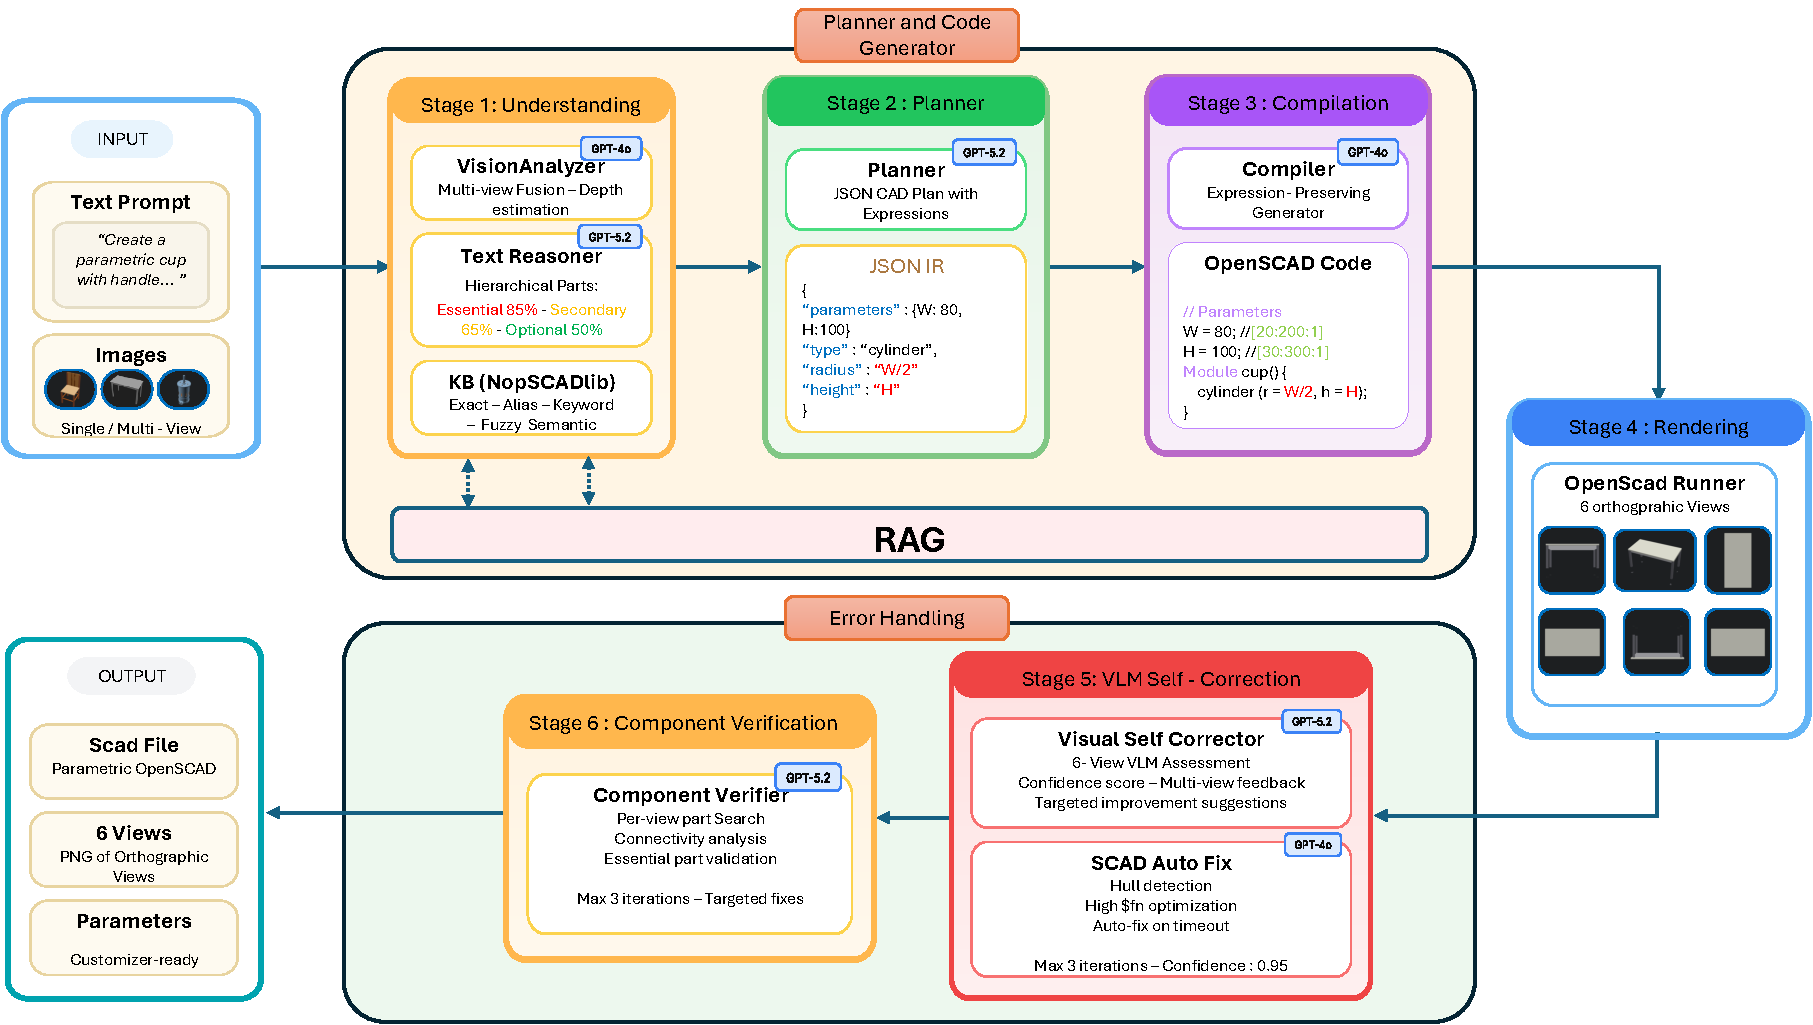
\includegraphics[width=0.99\linewidth]{figures/pdf/Craft_pipeline.pdf}
    \caption{Overview of the CRAFT pipeline. The system maps a text prompt and optional reference images to a parametric OpenSCAD program through six stages: understanding, planning, compilation, rendering, multi-view visual correction, and component verification. Reasoning-intensive stages use GPT-5.2, while deterministic translation and repair steps use GPT-4o.}
    \label{Fig:pipeline}
\end{figure*}


\textbf{Verification and Visual Feedback.} Recent work has begun to address correctness verification as a first-class concern in CAD generation. CADCodeVerify~\citep{alrashedy2024cadcodeverify} introduces vision-language model-based verification and iterative correction as a post-generation step, achieving measurable quality improvements without retraining. More broadly, visual feedback has emerged as a powerful signal for program repair: rendering a generated program and comparing the output against a reference provides information that is difficult to obtain from code analysis alone. CRAFT extends this direction by rendering six orthographic views rather than a single image, enabling the VLM to detect geometric errors that are invisible from any single viewpoint, and integrating this feedback within a bounded iterative correction loop rather than as a one-shot post-processing step.

\textbf{Retrieval-Augmented Generation.} Retrieval-augmented generation (RAG) has shown that grounding language model outputs in external knowledge sources improves both factual accuracy and domain specificity~\citep{lewis2020rag}. In the code-generation setting, retrieving relevant library components or API signatures at generation time can reduce hallucination and improve structural correctness. CRAFT applies this principle to parametric CAD by retrieving component specifications from NopSCADlib~\citep{nopscadlib} during the understanding stage, grounding generated geometry in catalog-defined dimensions rather than relying on the model's implicit knowledge of part geometries.

\textbf{Multi-Agent Systems.} Multi-agent pipelines have demonstrated advantages over single-model generation in tasks requiring planning, execution, and verification across multiple steps~\citep{guo2024multiagent}. Such systems can isolate failure modes and apply targeted repair without regenerating earlier stages by assigning specialized roles to distinct agents. This architecture is well-suited to CAD generation, where failures can occur at the planning, compilation, rendering, or geometric correctness levels, each requiring a different repair strategy. CRAFT adopts a six-stage multi-agent design in which each stage is independently recoverable, and coordinates these stages through a five-layer recovery strategy that escalates from cheap structural fixes to more costly semantic correction only when necessary.

\textbf{Parametric Modeling.} Parametric CAD represents geometry through symbolic variables and editable relationships rather than fixed coordinate values, enabling downstream customization, reuse, and engineering analysis~\citep{fusion360gallery2021,wu2021deepcad}. Despite this importance, most text-to-CAD systems emit hard-coded numeric geometry, discarding the symbolic structure that makes models practically useful. OpenSCAD~\citep{openscad} provides a natural target for preserving this structure through top-level parameter declarations and symbolic expressions. CRAFT is designed around this requirement: its JSON intermediate representation explicitly stores dimensions as symbolic strings, which are carried through compilation unchanged, ensuring that the final OpenSCAD programs remain fully editable.


\section{Methods}
\label{Sec:method}

CRAFT transforms natural language descriptions and optional reference images into parametric OpenSCAD code through six sequential stages. In our implementation, reasoning-intensive stages (understanding, planning, multi-view assessment, and component verification) are handled by a reasoning LLM (GPT-5.2), while deterministic translation and repair steps are handled by a traditional LLM (GPT-4o). The six stages describe the forward generation path, whereas the five recovery layers introduced in \secref{subSec:recovery} describe how the system escalates repair when intermediate artifacts are invalid or the rendered result is unsatisfactory. 

The pipeline (\figref{Fig:pipeline}) begins with understanding (Stage~1), where image and text inputs are processed in parallel. The image-analysis path extracts geometric cues from any provided reference images and fuses information across views when multiple images are available. The text-reasoning parses the prompt to identify required components, classify them by importance (essential, secondary, optional), and detect references to standard parts such as motors or fasteners. When such components are recognized, their specifications are retrieved from NopSCADlib~\citep{nopscadlib} using five strategies: exact name matching, fuzzy name matching, category-based lookup, dimensional attribute matching, and semantic embedding retrieval. If retrieval fails, the pipeline proceeds with LLM-only synthesis using a retrieve-then-generate design pattern~\citep{lewis2020rag}.

The output of stage~1 is passed to planning (Stage~2), where the planner produces a JSON CAD plan (Section~\ref{subSec:json-ir}). This intermediate representation encodes geometry, constructive solid geometry (CSG) operations, and symbolic parametric expressions in a structured format that can be validated before any code is generated. In compilation (Stage~3), the validated plan is translated into OpenSCAD that preserves expression strings and generates parameter ranges for the customizer interface.

In rendering (Stage~4), OpenSCAD produces six orthographic views: front, back, left, right, top, and bottom. The renderer also applies timeout-aware simplifications for computationally expensive constructs such as \texttt{hull()}, which can become slow when computing enclosing geometry over multiple primitives. These views are then used in VLM self-correction (Stage~5, Section~\ref{subSec:vlm}), where a vision-language model compares the rendered output against the original prompt and iteratively proposes fixes for up to three rounds. Finally, component verification (Stage~6) checks whether the expected parts are present using tiered confidence thresholds of 85\% for essential parts, 65\% for secondary parts, and 50\% for optional parts. These thresholds were set empirically during pilot runs to prioritize functionally necessary components over cosmetic details. This reflects the idea that missing mounting holes in a motor bracket constitute a failure, whereas omitting a cosmetic chamfer may still yield an acceptable design. More broadly, this iterative repair process is conceptually related to recent self-refinement approaches for large models~\citep{madaan2023selfrefine}.

\subsection{JSON Intermediate Representation}
\label{subSec:json-ir}

CRAFT uses a JSON intermediate representation (IR) between design understanding and OpenSCAD generation. The IR encodes parameters, geometric primitives, and CSG operations in a structured form that can be validated before compilation. Unlike direct code generation, the IR preserves symbolic parametric expressions rather than evaluating them into constants. Expressions such as \texttt{"outer\_diameter/2"} are passed directly into the compiled OpenSCAD code, allowing the final model to remain editable and fully parametric. 
%(\figref{Fig:json-to-scad}).

\subsection{Multi-View VLM Assessment}
\label{subSec:vlm}

Single-image assessment can miss geometric issues that are visible only from specific viewpoints. A model that appears correct from the front may still have incorrect depth or missing features visible only from the side. CRAFT addresses this by rendering six orthographic views (front, back, left, right, top, and bottom) and presenting them jointly to a vision-language model (VLM) for assessment. The VLM returns a confidence score on a 0--1 scale, a list of identified issues, and suggested corrections. If the confidence falls below 0.95, the system generates targeted fixes for the affected parts rather than regenerating the entire design. This loop runs for up to three iterations, with early stopping once the confidence threshold is reached. In our implementation, this assessment is performed using GPT-5.2 due to its stronger spatial reasoning capability.

\subsection{Layered Error Recovery}
\label{subSec:recovery}

The recovery layers describe how CRAFT escalates repair when intermediate artifacts fail validation, rendering, or semantic checks. Failures in text-to-CAD generation can arise at several levels: invalid intermediate plans, non-renderable code, and geometrically incorrect outputs. CRAFT addresses these through a five-layer strategy that orders repair mechanisms from inexpensive structural fixes to more costly semantic correction. The first layer repairs malformed JSON plans through schema validation and automatic repair. The second layer applies deterministic OpenSCAD fixes for common rendering failures, such as expensive operations or excessive mesh resolution. The third layer re-invokes the multi-view VLM assessment from Stage~5 to detect semantic and geometric mismatches and generate targeted corrections. The fourth layer re-invokes the component verification procedure from Stage~6 under the same tiered thresholds. The fifth layer incorporates manual repair hints when automatic recovery remains insufficient. Automatic recovery operates under a fixed retry budget of 10 total attempts across the first four layers, set empirically to balance correction capability against latency and cost. In the reported experiments, staged recovery resolved compilation and rendering failures before final output assessment, allowing the comparison to focus on geometric fidelity and semantic alignment of the final recovered outputs.

\section{Results}
\label{Sec:results}

We evaluate CRAFT against direct generation baselines using GPT-4o and GPT-5.2 to examine whether its structured design improves semantic alignment with the input prompt, geometric faithfulness, and robustness under challenging generation settings, while retaining editable parametric relationships rather than collapsing into fixed geometry. Experiments are conducted on the NopSCADlib benchmark and two additional datasets (ABC and Slice-100K) to assess both in-domain performance and cross-dataset generalization. Detailed experimental settings are provided in \secref{Sec:setup}.
% We organize the evaluation around the main design goals of CRAFT: perceptual alignment with the prompt, geometric fidelity of the generated shape, behavior under increasing prompt complexity, and robustness through bounded corrective recovery.


\subsection{Perceptual Alignment}

We first evaluate how well generated models match their text descriptions using CLIP Score and Fr\'echet Inception Distance (FID). CLIP Score measures semantic alignment between rendered CAD images and their prompts, while FID measures how closely the generated renderings match the distribution of ground-truth CAD images.

\begin{table}[t!]
    \centering
    \caption{Perceptual evaluation on NopSCADlib. CLIP Score measures text--image alignment (higher is better), while FID measures distributional similarity to ground-truth renders (lower is better). GT denotes the ground-truth CLIP score as a reference upper bound.}
    \label{tab:perceptual}
    \small
    \setlength{\tabcolsep}{4pt}
    \begin{tabular}{lcccc}
    \toprule
    Metric & CRAFT & GPT-4o & GPT-5.2 & GT \\
    \midrule
    CLIP Score & \textbf{0.2223} & 0.2033 & 0.2145 & 0.2333 \\
    \quad Simple & \textbf{0.2260} & 0.2098 & 0.2174 & 0.2279 \\
    \quad Medium & \textbf{0.2159} & 0.2014 & 0.2144 & 0.2317 \\
    \quad Complex & \textbf{0.2251} & 0.1983 & 0.2116 & 0.2409 \\
    \midrule
    FID & \textbf{94.47} & 118.01 & 104.63 & --- \\
    \quad Simple & 154.65 & 144.85 & \textbf{136.43} & --- \\
    \quad Medium & \textbf{130.33} & 155.06 & 143.33 & --- \\
    \quad Complex & \textbf{136.90} & 184.38 & 160.51 & --- \\
    \bottomrule
    \end{tabular}
\end{table}



\tabref{tab:perceptual} shows that CRAFT achieves the strongest overall perceptual alignment on NopSCADlib. CRAFT reaches a mean CLIP score of 0.2223, which is the highest among the compared methods and closest to the ground-truth reference score of 0.2333. This advantage is maintained across all three complexity tiers, indicating that the structured pipeline helps preserve the semantic intent of the prompt consistently rather than only on simpler examples. FID follows a similar overall trend. CRAFT achieves the lowest overall FID of 94.47, compared to 104.63 for GPT-5.2 and 118.01 for GPT-4o, suggesting that its generated shapes more closely match the visual distribution of the reference CAD models. The gap becomes more pronounced on medium and complex components, where structured planning, component retrieval, and iterative verification appear to better preserve global shape organization. On simple components, GPT-5.2 achieves the lowest FID, suggesting that direct generation can be effective for basic geometry, while the advantage of CRAFT becomes more apparent as design difficulty increases.




\subsection{Geometric Accuracy}

We next evaluate geometric fidelity using Chamfer Distance (CD), F1, and voxel IoU. F1 score is reported at a 1\% distance threshold. These metrics measure complementary aspects of reconstruction quality, including surface proximity, point-level matching, and volumetric overlap with ground-truth models. 


\begin{table}[t!]
    \centering
    \caption{Geometric evaluation on NopSCADlib, including overall results and breakdown by prompt complexity. F1 is reported at a 1\% distance threshold. Best results in each row group are shown in bold.}
    \label{tab:nopscad-results}
    \small
    \setlength{\tabcolsep}{6pt}
    \begin{tabular}{llccc}
    \toprule
    Split & Method & CD$\downarrow$ & F1$\uparrow$ & Voxel IoU$\uparrow$ \\
    \midrule
    \multirow{3}{*}{Overall}
    & CRAFT   & 0.0704 & 0.2369 & \textbf{0.2242} \\
    & GPT-4o  & 0.0742 & 0.2467 & 0.2182 \\
    & GPT-5.2 & \textbf{0.0671} & \textbf{0.2585} & 0.1870 \\
    \midrule
    \multirow{3}{*}{Simple}
    & CRAFT   & 0.0941 & 0.3054 & 0.2529 \\
    & GPT-4o  & 0.0840 & 0.3424 & \textbf{0.3475} \\
    & GPT-5.2 & \textbf{0.0788} & \textbf{0.3480} & 0.1567 \\
    \midrule
    \multirow{3}{*}{Medium}
    & CRAFT   & \textbf{0.0563} & 0.2256 & 0.2450 \\
    & GPT-4o  & 0.0650 & 0.2253 & 0.1807 \\
    & GPT-5.2 & 0.0583 & \textbf{0.2342} & \textbf{0.2536} \\
    \midrule
    \multirow{3}{*}{Complex}
    & CRAFT   & \textbf{0.0593} & 0.1744 & \textbf{0.1712} \\
    & GPT-4o  & 0.0737 & 0.1677 & 0.1207 \\
    & GPT-5.2 & 0.0638 & \textbf{0.1871} & 0.1500 \\
    \bottomrule
    \end{tabular}
\end{table}


\begin{table}[t!]
\centering
\caption{Geometric evaluation on ABC, including overall results and breakdown by prompt complexity. F1 is reported at a 1\% distance threshold. Best results in each row group are shown in bold.}
\label{tab:abc-results}
\small
\setlength{\tabcolsep}{6pt}
\begin{tabular}{llccc}
\toprule
Split & Method & CD$\downarrow$ & F1$\uparrow$ & Voxel IoU$\uparrow$ \\
\midrule
\multirow{3}{*}{Overall}
& CRAFT   & \textbf{0.0804} & \textbf{0.1303} & \textbf{0.0401} \\
& GPT-4o  & 0.1009 & 0.0847 & 0.0211 \\
& GPT-5.2 & 0.0950 & 0.0880 & 0.0187 \\
\midrule
\multirow{3}{*}{Simple}
& CRAFT   & \textbf{0.0825} & \textbf{0.1538} & \textbf{0.0353} \\
& GPT-4o  & 0.0978 & 0.0778 & 0.0288 \\
& GPT-5.2 & 0.0903 & 0.0942 & 0.0148 \\
\midrule
\multirow{3}{*}{Medium}
& CRAFT   & \textbf{0.0701} & \textbf{0.1137} & \textbf{0.0325} \\
& GPT-4o  & 0.0994 & 0.0947 & 0.0152 \\
& GPT-5.2 & 0.0936 & 0.0946 & 0.0146 \\
\midrule
\multirow{3}{*}{Complex}
& CRAFT   & \textbf{0.0884} & \textbf{0.1244} & \textbf{0.0519} \\
& GPT-4o  & 0.1059 & 0.0828 & 0.0180 \\
& GPT-5.2 & 0.1006 & 0.0762 & 0.0261 \\
\bottomrule
\end{tabular}
\end{table}

\begin{table}[t!]
\centering
\caption{Geometric evaluation on Slice-100K, including overall results and breakdown by prompt complexity. F1 is reported at a 1\% distance threshold. Best results in each row group are shown in bold.}
\label{tab:slice-results}
\small
\setlength{\tabcolsep}{6pt}
\begin{tabular}{llccc}
\toprule
Split & Method & CD$\downarrow$ & F1$\uparrow$ & Voxel IoU$\uparrow$ \\
\midrule
\multirow{3}{*}{Overall}
& CRAFT   & 0.0617 & \textbf{0.2831} & 0.0633 \\
& GPT-4o  & 0.0743 & 0.2146 & \textbf{0.0718} \\
& GPT-5.2 & \textbf{0.0607} & 0.2828 & 0.0627 \\
\midrule
\multirow{3}{*}{Simple}
& CRAFT   & \textbf{0.0414} & \textbf{0.4018} & \textbf{0.0763} \\
& GPT-4o  & 0.0601 & 0.2976 & 0.0537 \\
& GPT-5.2 & 0.0439 & 0.3770 & 0.0609 \\
\midrule
\multirow{3}{*}{Medium}
& CRAFT   & 0.0752 & 0.1918 & 0.0428 \\
& GPT-4o  & 0.0783 & 0.1026 & 0.0498 \\
& GPT-5.2 & \textbf{0.0631} & \textbf{0.2364} & \textbf{0.0579} \\
\midrule
\multirow{3}{*}{Complex}
& CRAFT   & \textbf{0.0682} & \textbf{0.2565} & 0.0706 \\
& GPT-4o  & 0.0837 & 0.2417 & \textbf{0.1094} \\
& GPT-5.2 & 0.0743 & 0.2366 & 0.0687 \\
\bottomrule
\end{tabular}
\end{table}


\tabref{tab:nopscad-results}, \tabref{tab:abc-results}, and \tabref{tab:slice-results} summarize geometric results on NopSCADlib, ABC, and Slice-100K, respectively. On ABC, CRAFT achieves the strongest overall performance across all three metrics, obtaining the lowest CD, highest F1, and highest voxel IoU, suggesting that the structured intermediate representation and layered recovery improve generalization to unfamiliar geometry. On Slice-100K, results are more comparable: GPT-5.2 achieves the lowest CD, CRAFT achieves the highest F1, and GPT-4o attains the highest voxel IoU despite weaker surface-based metrics. On NopSCADlib, GPT-5.2 leads on CD and F1 while CRAFT achieves the highest voxel IoU, indicating that direct generation can yield slightly better average surface proximity on in-distribution examples, whereas CRAFT produces stronger volumetric consistency. Taken together with the perceptual results, CRAFT is particularly effective at producing geometrically coherent parametric models rather than optimizing any single surface metric in isolation.

\subsection{Effect of Complexity}

We break down results by prompt complexity to examine how performance varies with design difficulty. On NopSCADlib, direct generation remains highly competitive on simple components: GPT-5.2 achieves the lowest CD and highest F1, while GPT-4o attains the highest voxel IoU. When prompts describe basic geometry with limited part interactions, direct code synthesis often produces acceptable models. As complexity increases, CRAFT's advantage becomes more apparent. On medium-complexity examples, CRAFT achieves the lowest CD, though GPT-5.2 remains slightly stronger on F1 and voxel IoU. On complex examples involving multiple interacting features such as mounting holes, flanges, or internal cutouts, CRAFT achieves the lowest CD and highest voxel IoU. Although GPT-5.2 retains an advantage in F1 on medium and complex tiers, CRAFT shows more consistent geometric behavior as structural difficulty increases. On ABC, CRAFT achieves the best CD, F1, and voxel IoU at every complexity tier, with especially pronounced margins on complex components, indicating consistent generalization across prompt difficulty on previously unseen geometry.

% On Slice-100K, the pattern is more mixed: CRAFT leads on simple and complex tiers in CD and F1, while GPT-5.2 performs best across all three metrics on the medium tier, and GPT-4o attains the highest voxel IoU on complex components.

Overall, these results support the design motivation behind CRAFT. Structured planning and layered recovery offer limited advantage on simple targets, but become increasingly useful when prompts require multiple relations, reusable dimensions, coordinated part composition, and recovery from intermediate errors.

\subsection{Robustness and Recovery Behavior}
\label{subSec:robustness}

Beyond final-shape quality, CRAFT is designed to improve robustness through bounded staged recovery rather than relying on a single forward generation pass. In the main evaluation, we report only the quality of the final recovered outputs, not per-stage failure counts. As a result, the geometric and perceptual gains in Tables~\ref{tab:perceptual}--\ref{tab:slice-results} should be interpreted primarily as end-to-end outcome quality after recovery, rather than as isolated measurements of intermediate compilation or repair success. Even under this conservative view, the stronger performance of CRAFT on medium-complexity, complex, and out-of-distribution examples is consistent with the role of structured planning and targeted correction in stabilizing generation when direct one-shot synthesis becomes brittle.

This robustness mechanism is especially important for text-to-parametric CAD, where failure can occur at multiple levels: malformed intermediate plans, non-renderable OpenSCAD code, incomplete part composition, or geometry that is syntactically valid but semantically inconsistent with the prompt. CRAFT addresses these failure modes through schema-level repair, deterministic OpenSCAD fixes, multi-view VLM-guided correction, and component-level verification within a bounded retry budget. Expanded qualitative illustrations of this layered recovery process and its role in improving generation stability are provided in the appendix.

\subsection{Preservation of Parametric Relationships}
\label{subSec:parametric_relationships}

Beyond perceptual and geometric quality, we also examine whether the generated CAD programs preserve editable parametric structure. \figref{Fig:parametric_edits} shows representative examples where changing individual parameters produces coherent geometric and appearance changes. This indicates that CRAFT generates executable parametric programs rather than only fixed shape approximations.

\begin{figure}[t]
    \centering
    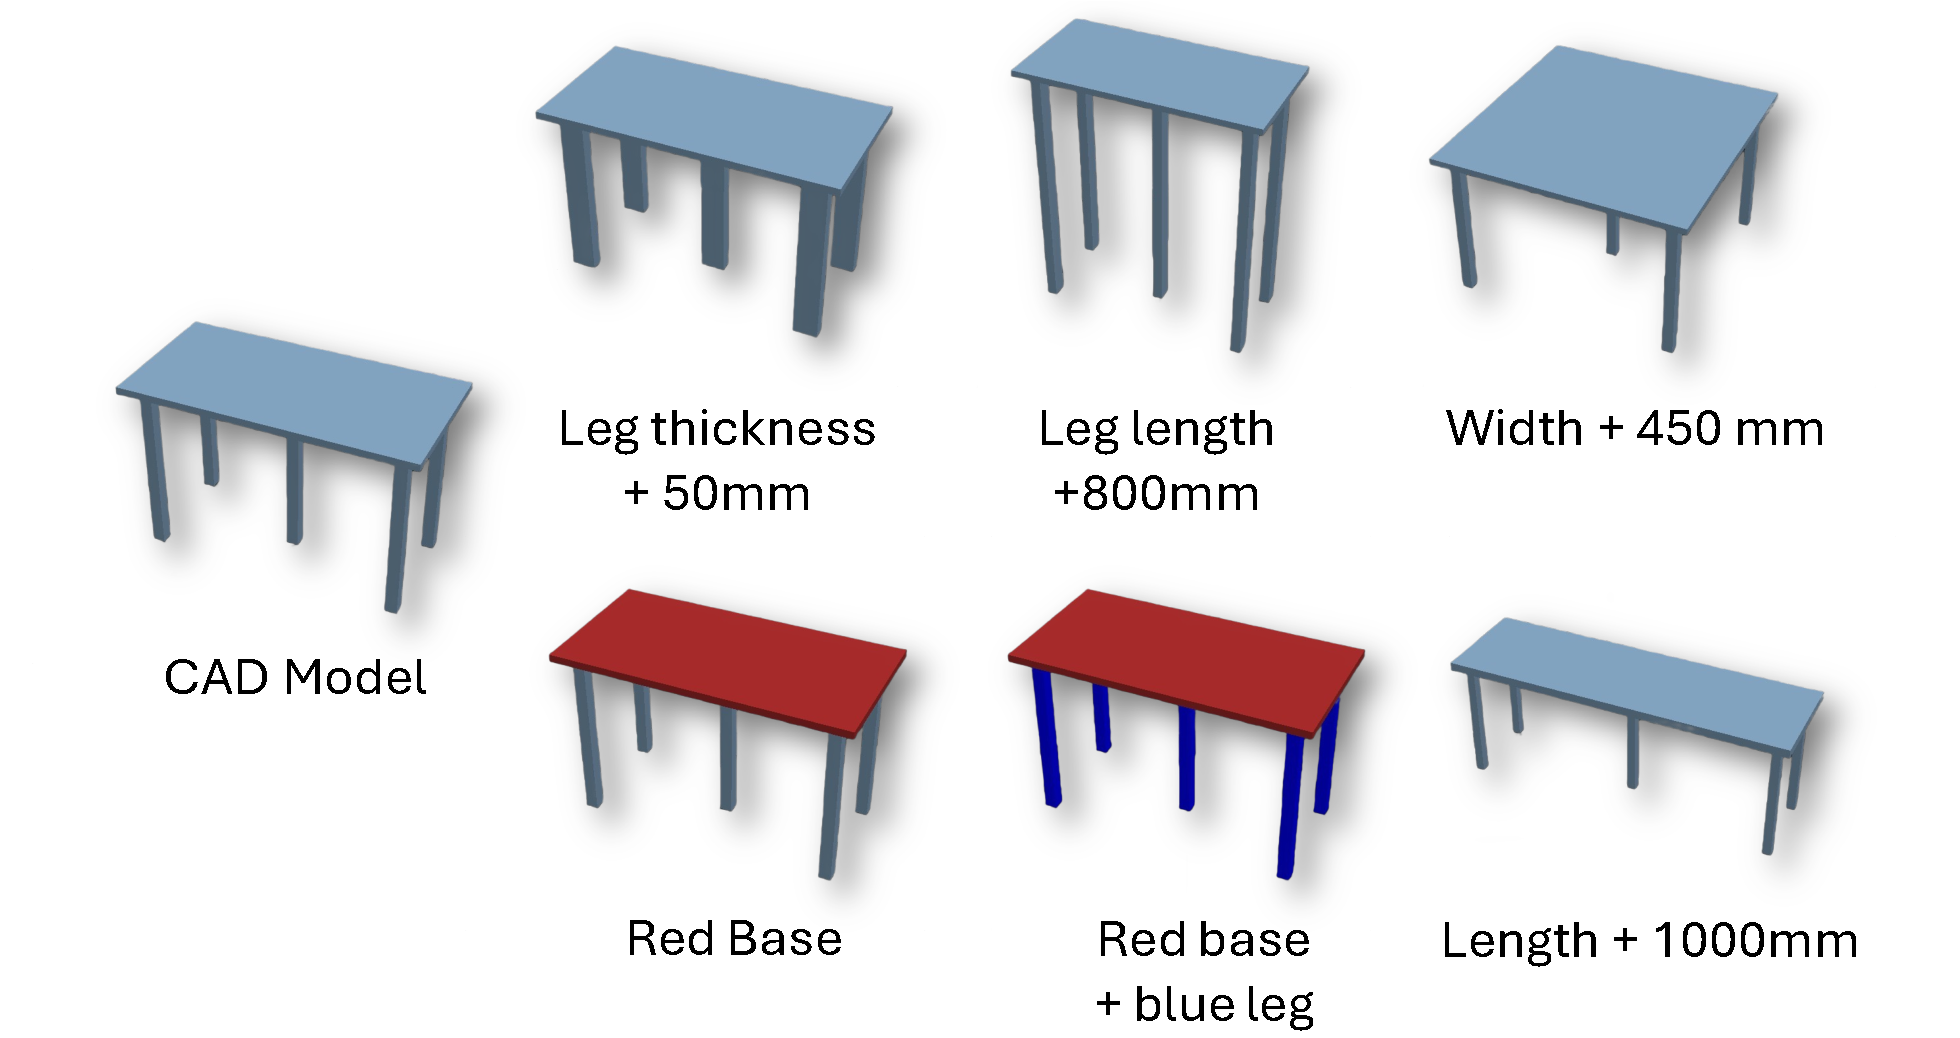
\includegraphics[width=\linewidth]{figures/pdf/Parametric_Cad_Example.pdf}
\caption{Examples of preserved parametric editability in generated CAD models. Changing individual parameters produces coherent geometric and appearance variations, showing that the generated OpenSCAD programs retain interpretable parametric relationships rather than only fixed final shapes.}
    \label{Fig:parametric_edits}
\end{figure}


\section{Discussion}
\label{Sec:discussion}

CRAFT achieves consistent improvements over direct one-shot generation across multiple datasets and object categories, with the largest gains on medium and complex designs. This result confirms that structured generation becomes more valuable as geometric dependencies and design complexity grow. The JSON intermediate representation is central to this behavior: it preserves symbolic parametric intent before code synthesis, ensuring that generated programs retain meaningful design controls rather than collapsing into fixed geometry. The qualitative parameter-edit results directly support this interpretation.

Several \textbf{limitations} should be noted. Performance declines as complexity increases, particularly when shapes involve many interacting parts or implicit structural relationships that are difficult to infer from text alone. OpenSCAD, while well suited for symbolic parametric modeling, does not capture the feature-history richness of industrial CAD systems such as Fusion 360 Gallery~\citep{fusion360gallery2021}. The multi-stage pipeline also depends on external language and vision models, increasing inference cost and introducing the risk of error propagation across stages. Finally, the evaluation covers three datasets, which represents only a subset of real-world engineering designs.

% These limitations point to several directions for future work. Extending the intermediate representation to support richer constraints, assemblies, and feature-level operations would broaden the range of producible designs. Stronger geometry-aware verification could improve faithfulness beyond image-based consistency alone, and integrating CRAFT with more expressive CAD backends would enable downstream editing in feature-based modeling environments.

\section{Conclusions}
\label{Sec:conclusion}

We presented CRAFT, a multi-agent pipeline for text-to-parametric CAD generation that combines structured reasoning, a JSON-based intermediate representation, visual verification, and layered error recovery. Unlike direct code-generation approaches, CRAFT explicitly preserves symbolic parametric relationships during generation, producing OpenSCAD programs that are executable, editable, and reusable. Experiments across three datasets show that CRAFT achieves strong perceptual and geometric quality while maintaining high reliability. The results demonstrate that preserving parametric intent through an explicit intermediate structure is both feasible and consequential for practical CAD systems.

% , and that agentic pipelines offer a promising path toward more accessible, controllable, and engineering-aware design systems.

\clearpage
{
\small
\bibliographystyle{IEEEtran}
\bibliography{Refs}
}


\clearpage
% \appendix
\renewcommand{\thefigure}{A.\arabic{figure}}
\renewcommand{\thesection}{A.\roman{section}}
\setcounter{figure}{0}
\setcounter{table}{0}
\setcounter{section}{0}

\section{Experimental Setup}
\label{Sec:setup}

\textbf{Datasets.} We evaluate CRAFT on three datasets totaling 668 components to assess both in-domain performance and cross-dataset generalization. Our primary benchmark is NopSCADlib~\citep{nopscadlib}, comprising 468 text--CAD pairs derived from parametric OpenSCAD components in the NopSCADlib mechanical library. Ground-truth models are derived from catalog-defined parametric specifications in the library, providing reference geometry anchored in standard mechanical dimensions. To test generalization beyond the primary benchmark library, we also evaluate on 100 shapes from ABC~\citep{koch2019abc} and 100 shapes from Slice-100K~\citep{slice100k2024}. These external datasets contain geometry outside the NopSCADlib library and therefore provide a more challenging test of whether the pipeline can synthesize coherent parametric programs for previously unseen shapes.

\textbf{Prompt Complexity.} For each dataset, components are grouped into Simple, Medium, and Complex tiers to study how generation quality changes with design difficulty. For NopSCADlib, tiers are assigned by source code analysis: a weighted composite of seven structural features---primitive count ($\times1.0$), boolean operations ($\times1.5$), CSG depth ($\times0.5$), parameter count ($\times0.3$), sub-module calls ($\times2.0$), lines of code ($\times0.05$), and transform count ($\times0.3$)---split at the 33rd and 66th percentiles (boundaries: 36.50 and 66.25). These weights were chosen heuristically based on pilot inspection of code complexity and are intended only to define relative within-dataset difficulty tiers. This yields 159 Simple, 160 Medium, and 149 Complex components. For ABC and Slice-100K, where source code is unavailable, tiers are assigned by mesh geometry analysis using five features: face count (0.25), connected components (0.15), convex hull ratio (0.25), surface-to-bounding-box ratio (0.20), and compactness (0.15), with the same percentile-based splitting. These weights were likewise chosen heuristically to induce relative geometric difficulty groupings within each dataset. Because the NopSCADlib and external datasets use different feature spaces, these tiers should be interpreted as relative within-dataset groupings rather than directly comparable across datasets.

\textbf{Baselines.} We compare CRAFT against single-stage direct generation baselines using GPT-4o and GPT-5.2. Both baselines receive the same text prompt used by CRAFT along with a system prompt instructing the model to output only valid, executable OpenSCAD code. Generation uses temperature~$0.0$ (deterministic) in a single API call, with no intermediate JSON planning, no component retrieval, no visual feedback, and no error recovery. This comparison isolates the benefit of CRAFT's staged parametric planning and multi-layer recovery over direct code generation from the same underlying model family~\citep{openai2023gpt4}.

\textbf{CRAFT Configuration.} CRAFT uses a hybrid model allocation: GPT-5.2 for reasoning-intensive stages (understanding, planning, VLM self-correction, component verification) and GPT-4o for deterministic stages (compilation, repair). The planner is allowed up to 2 schema-repair attempts. VLM self-correction runs for up to 3 iterations with early stopping at confidence~$>0.95$, and component verification permits up to 3 iterations with tiered thresholds (Essential~85\%, Secondary~65\%, Optional~50\%). Temperature is set to $0.0$ for deterministic compilation and $0.7$ for planning-oriented stages.

\textbf{Metrics.} We report both geometric and perceptual metrics. For geometric evaluation, we compute bidirectional Chamfer Distance~\citep{fan2017pointset}:
\begin{equation}
\begin{aligned}
\operatorname{CD}
= \frac{1}{2} \Bigl(
&\operatorname{mean}\!\left(d_{\mathrm{gt}\to\mathrm{pred}}\right) 
&+ \operatorname{mean}\!\left(d_{\mathrm{pred}\to\mathrm{gt}}\right)
\Bigr).
\end{aligned}
\end{equation}
% \begin{equation}
%     d_{CD}(S_1, S_2) = \frac{1}{|S_1|}\sum_{x\in S_1}\min_{y\in S_2}||x-y||_2^2 + \frac{1}{|S_2|}\sum_{y\in S_2}\min_{x\in S_1}||x-y||_2^2
%     \end{equation}
which captures both accuracy (predictions close to ground truth) and coverage (ground truth adequately represented); F1 at a 1\% distance threshold; and voxel IoU measuring volumetric overlap. Point clouds of 10{,}000 points are sampled from each mesh for CD and F1 computation; voxelization uses a $64^3$ grid along the longest axis. For perceptual evaluation, we report CLIP score using ViT-L/14~\citep{radford2021clip} to measure text--image semantic alignment, and Fr\'echet Inception Distance (FID)~\citep{heusel2017fid} computed from 2048-dimensional features extracted at the average-pooling layer of Inception-v3 to measure distributional similarity between generated and ground-truth renders.


\textbf{Rendering and Evaluation Protocol.} For each method, the generated OpenSCAD program is compiled and rendered into multi-view images for perceptual evaluation, and the resulting geometry is exported to STL and converted into point clouds and voxel grids for geometric comparison against reference models. OpenSCAD renders all models at $512\times512$ resolution. STL export uses a 300\,s timeout and PNG rendering uses a 120\,s timeout to accommodate complex CSG operations. Six orthographic views (front, back, left, right, top, bottom) are rendered for VLM assessment and perceptual metric computation. CRAFT follows the full staged pipeline described in \secref{Sec:method}, while baselines output a single OpenSCAD file evaluated using the identical metric pipeline. All methods are evaluated over the same set of prompts. When a method fails to produce a valid output under the evaluation protocol, the example is assigned worst-case metric values so that invalid generations remain reflected in the aggregate results.


\section{Extended Ablation Studies}
\label{app:ablation}

% The ablation results in \tabref{tab:ablation-model-config}--\tabref{tab:component-verification} provide a complementary view of CRAFT not captured by dataset-level geometric metrics. 
In particular, they show that the hybrid configuration improves component completeness, that multi-view correction contributes most strongly in the first two rounds, and that tiered part verification preferentially preserves functionally important components.

\section{Layered Recovery and Multi-View Assessment}
\label{app:recovery}

\figref{fig:recovery-layers} and \figref{fig:multiview-assessment} illustrate two mechanisms most responsible for CRAFT's robustness: bounded layered repair and six-view visual feedback. These mechanisms are included here in expanded form because they are central to the engineering behavior of the system, but too detailed for the space-limited main paper.

\begin{figure}[t]
    \centering
    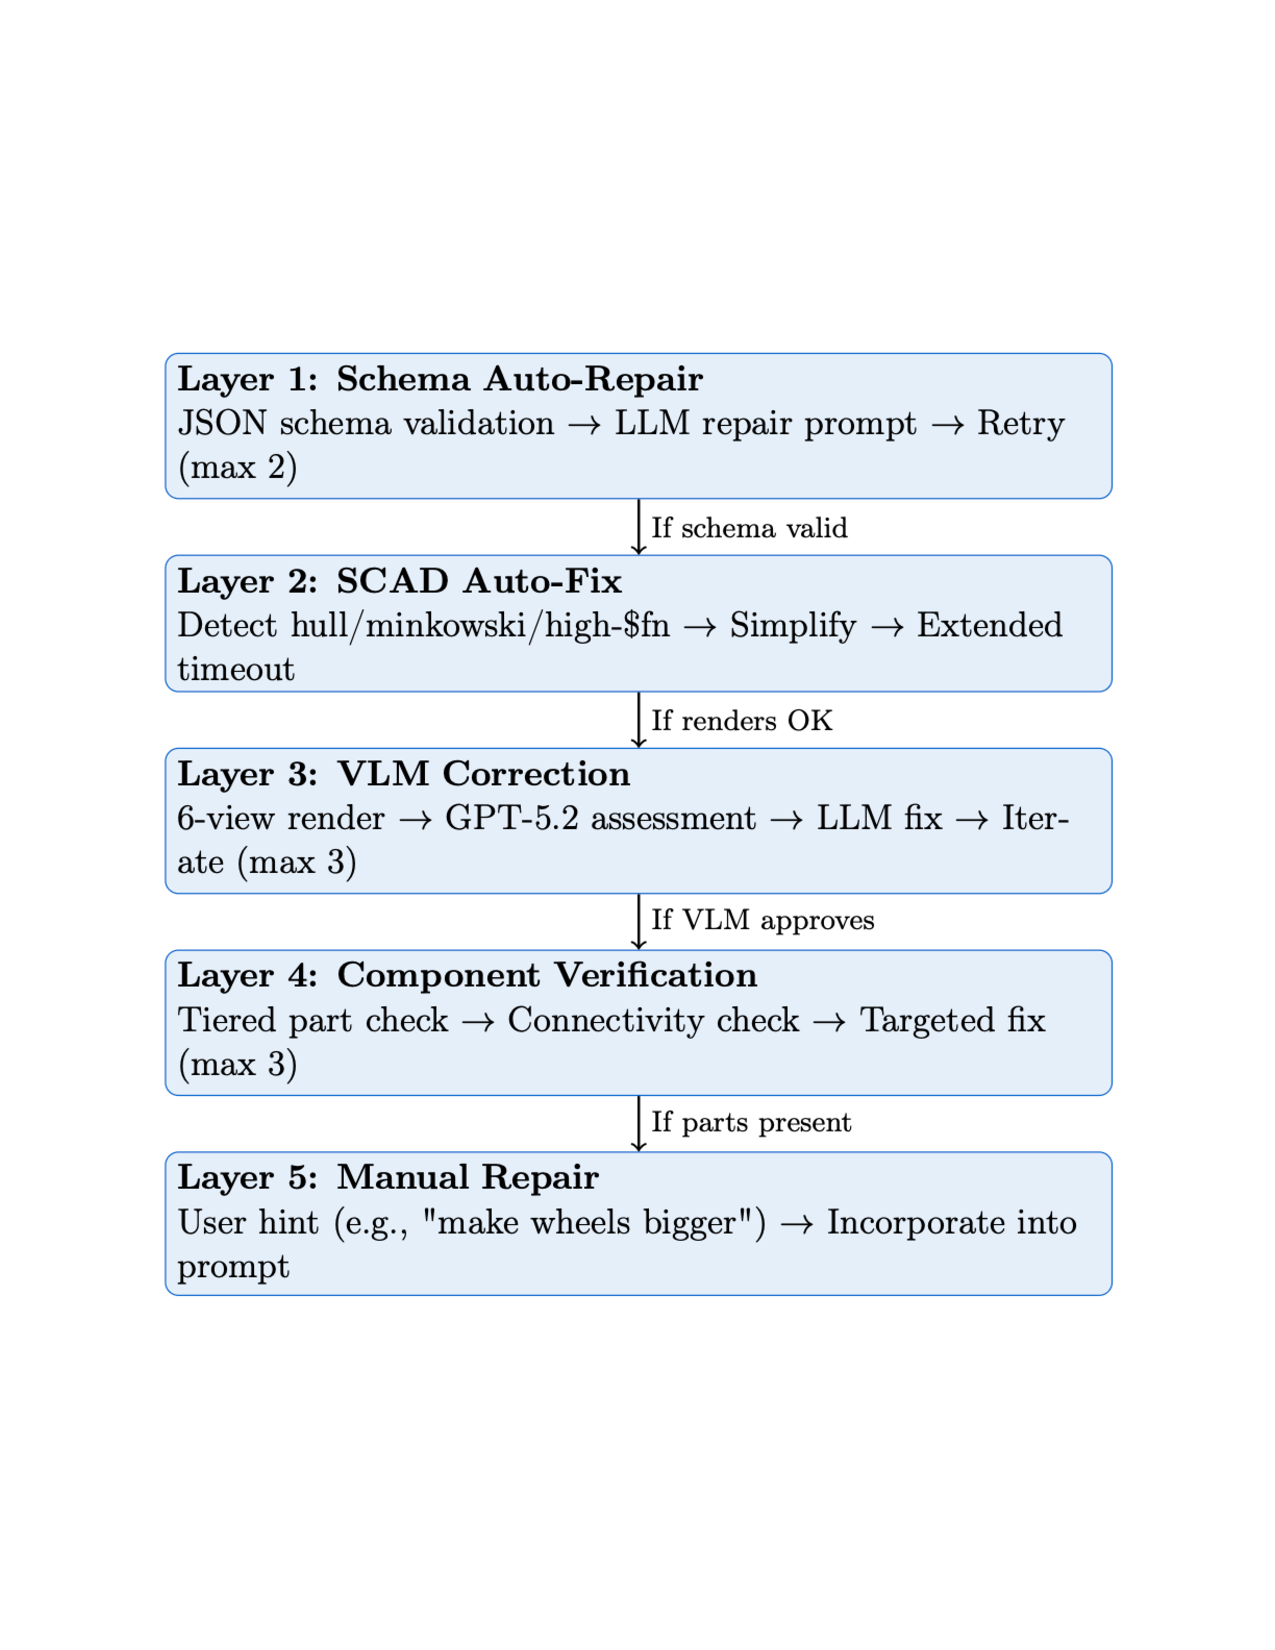
\includegraphics[width=0.99\linewidth,trim={1in 2.3in 1in 2.3in},clip]{figures/pdf/Error_correction_system.pdf}
    \caption{Expanded view of the layered recovery strategy used in CRAFT. The recovery process progresses through five stages: schema auto-repair, SCAD auto-fix, multi-view VLM correction, component verification, and optional manual repair. Repairs proceed from inexpensive structural fixes to increasingly semantic correction, with bounded retry budgets at intermediate stages.}
    \label{fig:recovery-layers}
\end{figure}


\begin{figure*}[t]
    \centering
    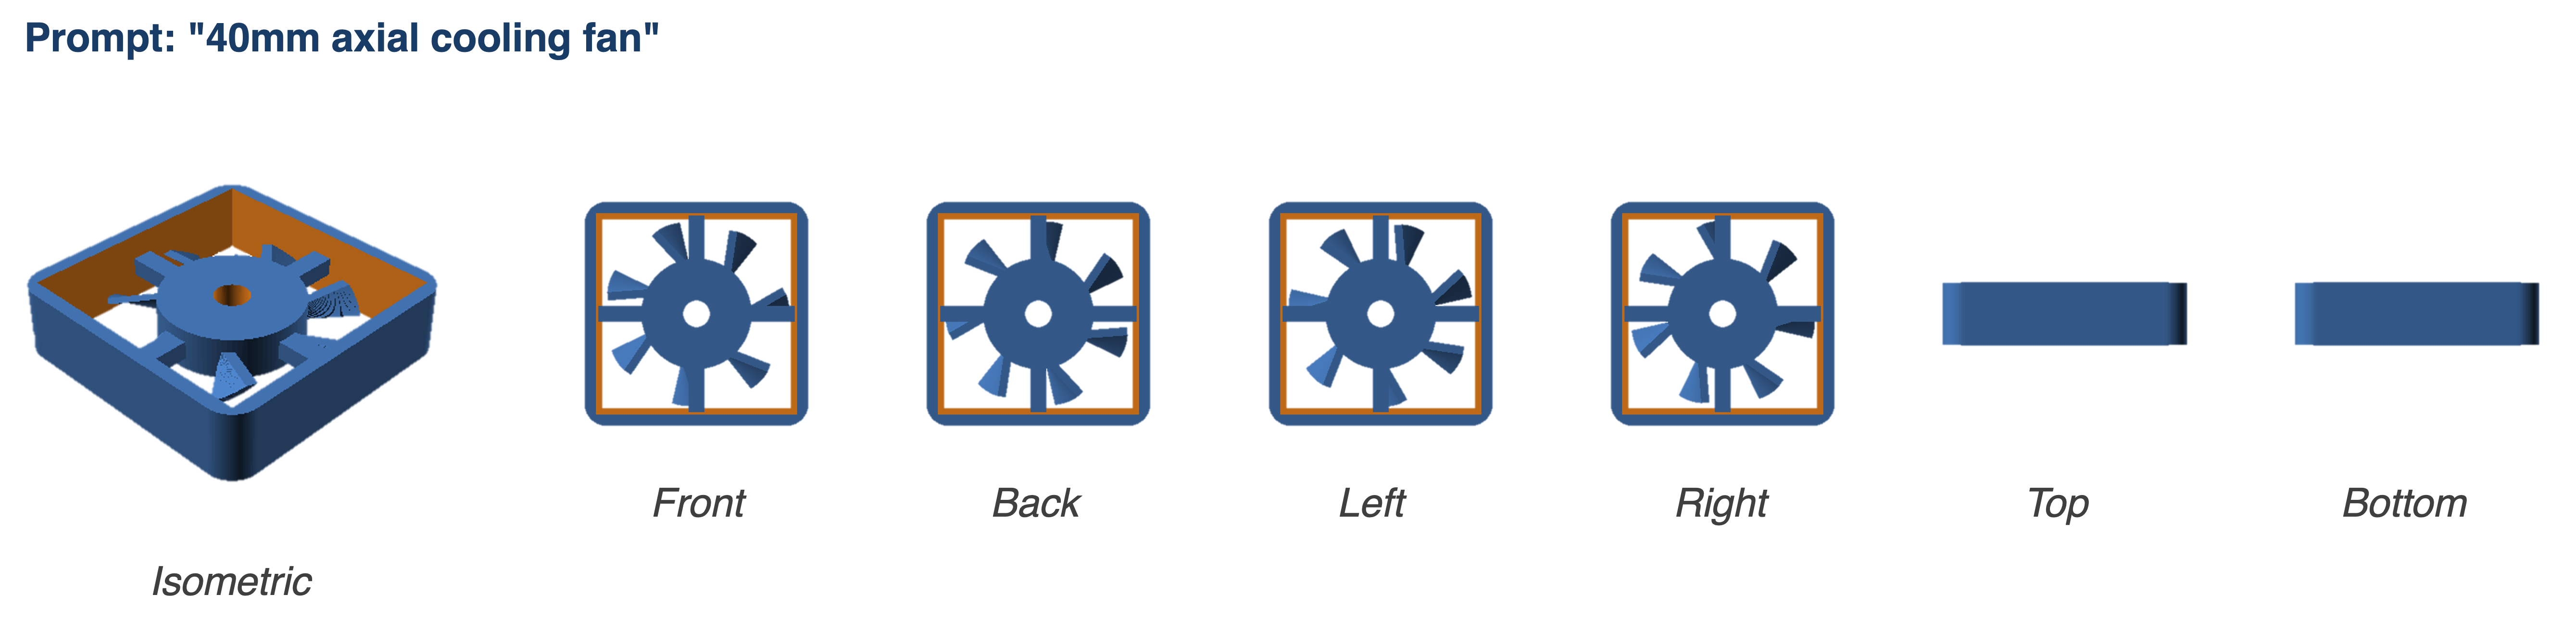
\includegraphics[width=0.8\linewidth]{figures/composites/Cooling_fan.png}
    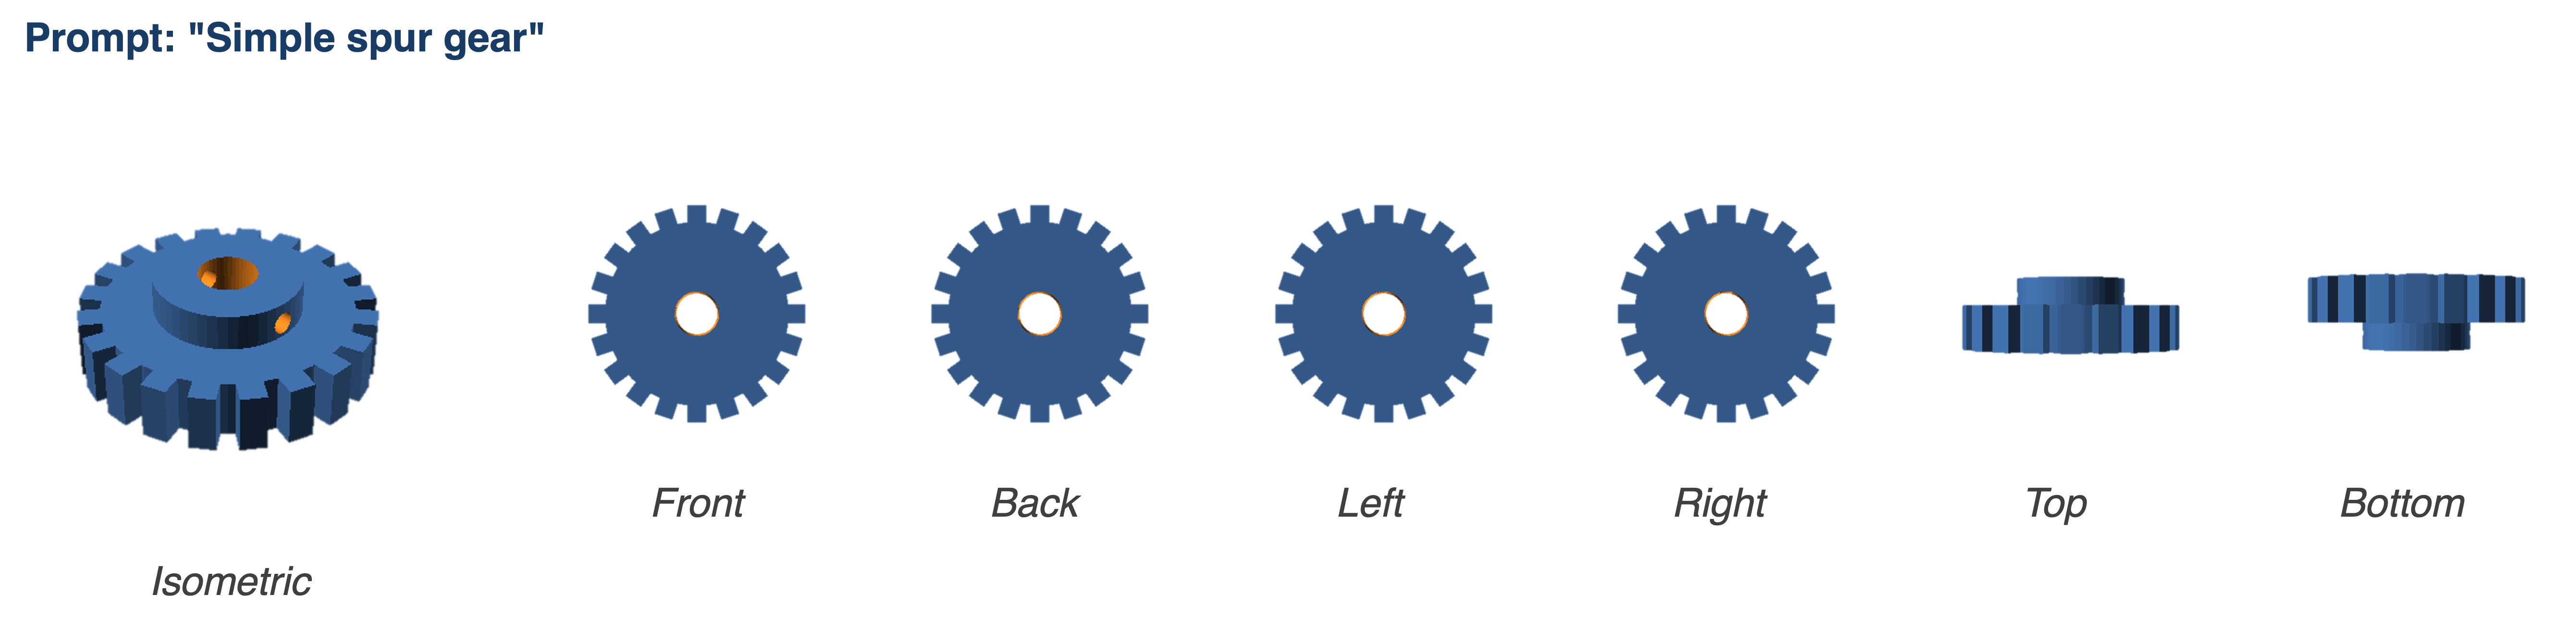
\includegraphics[width=0.8\linewidth]{figures/composites/Spur_gear.png}
    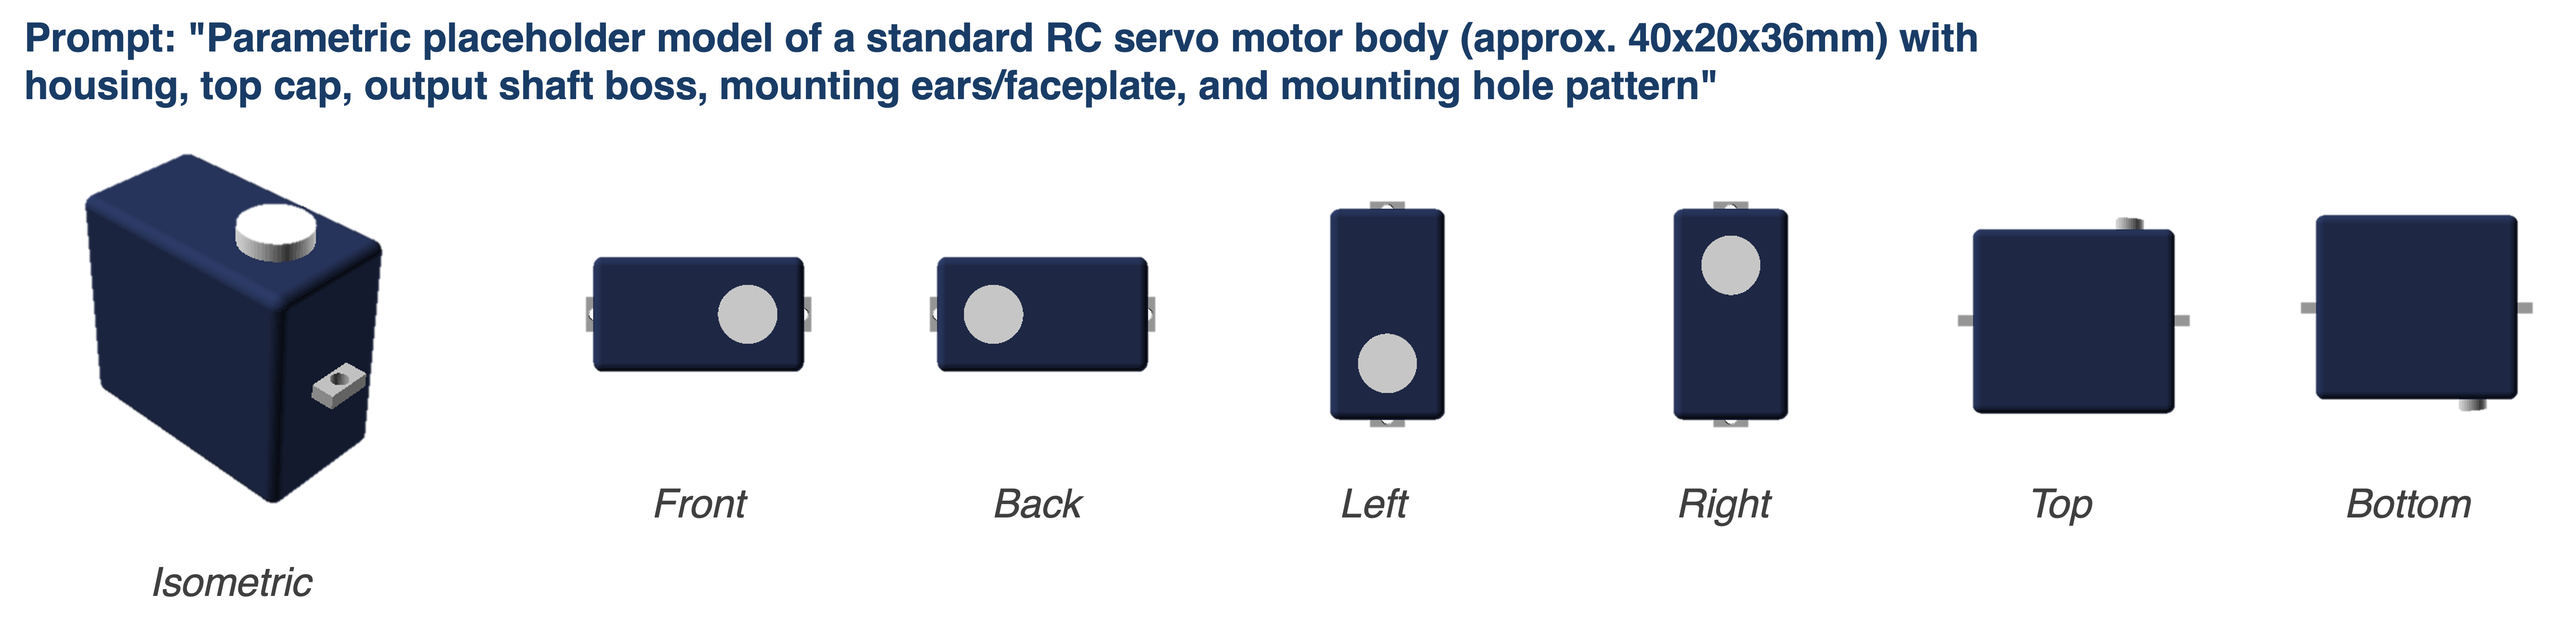
\includegraphics[width=0.8\linewidth]{figures/composites/RC_motor.png}
    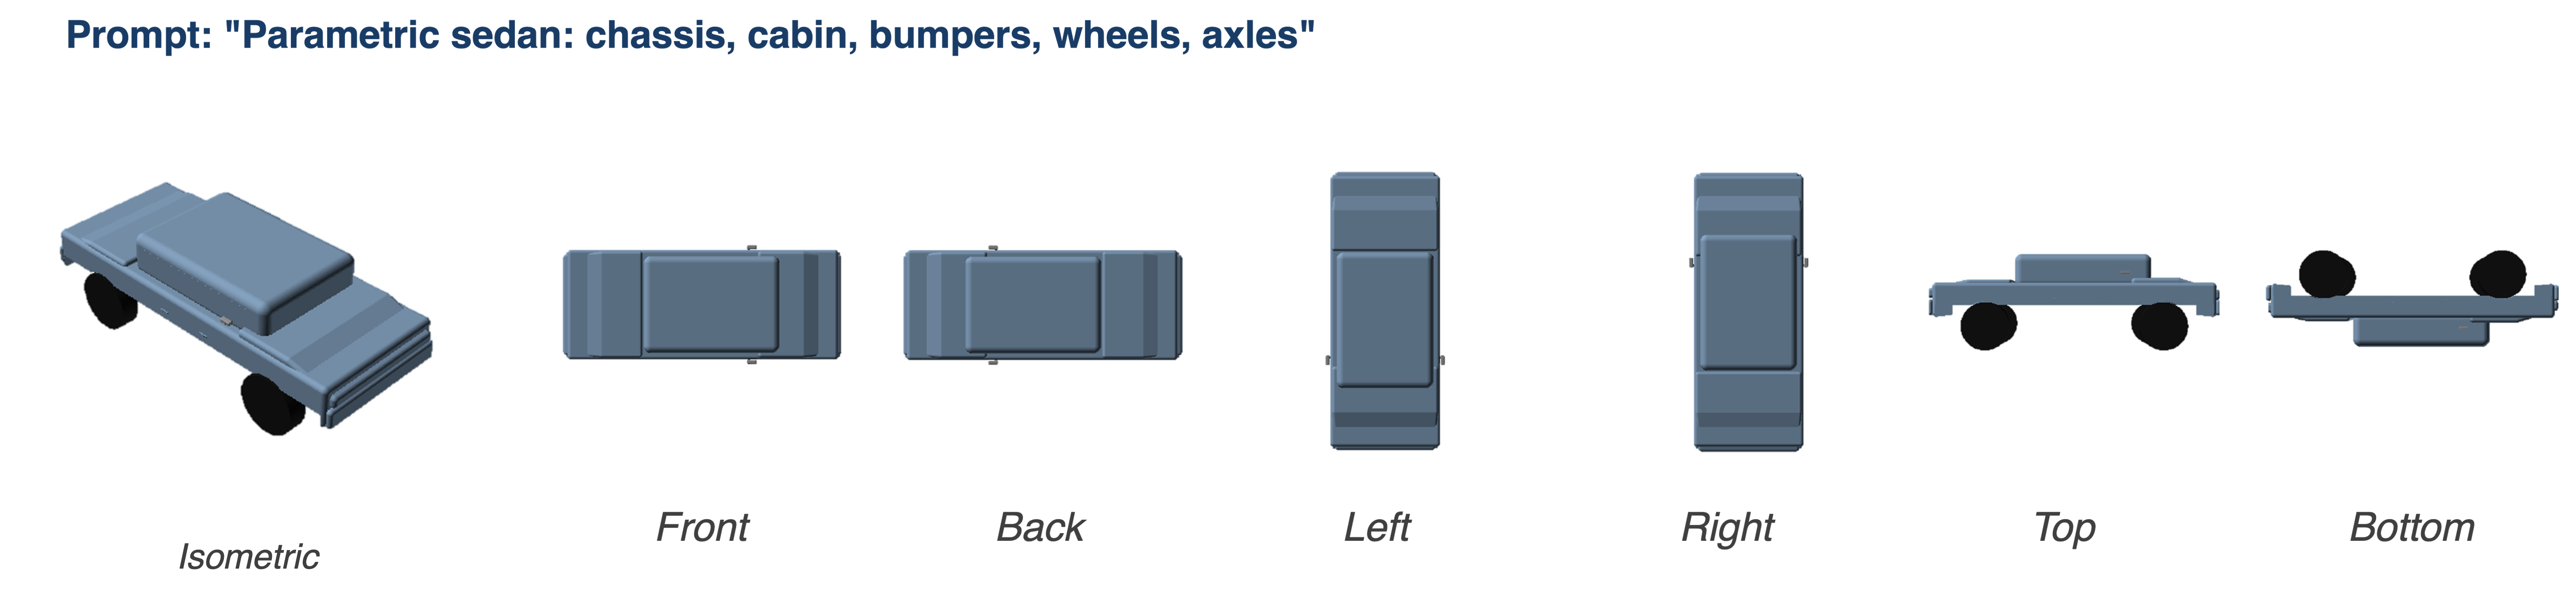
\includegraphics[width=0.8\linewidth]{figures/composites/sedan_car.png}
    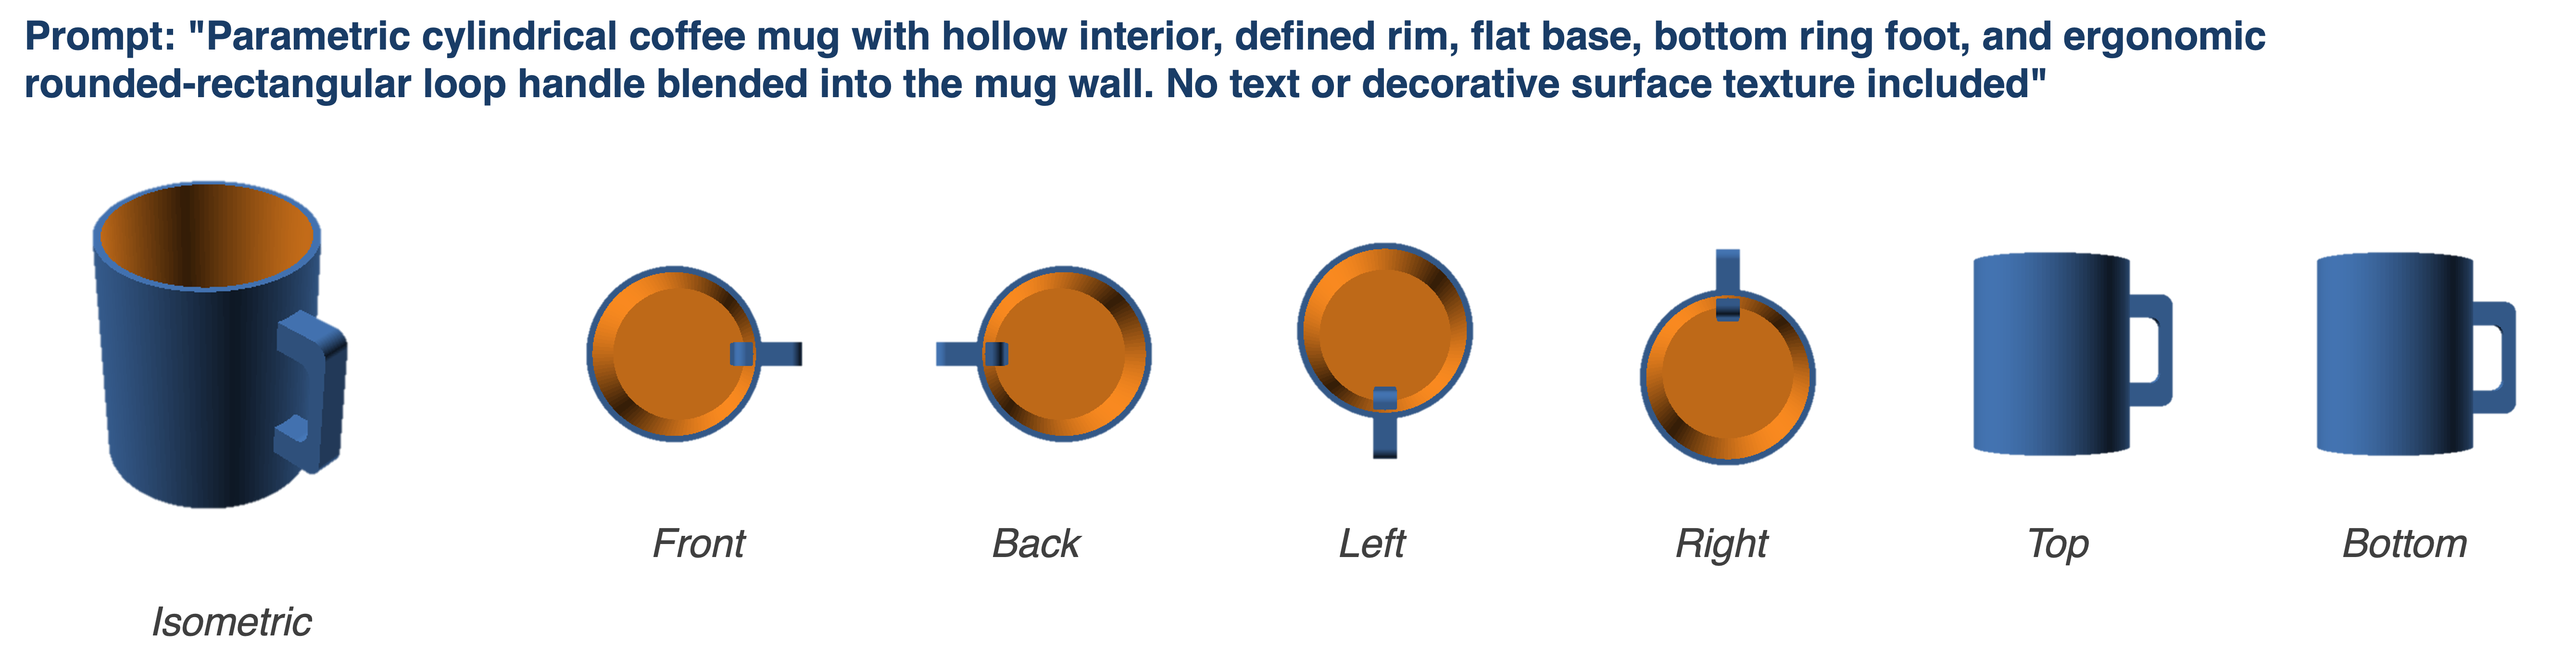
\includegraphics[width=0.8\textwidth]{figures/composites/Coffee_mug.png}
    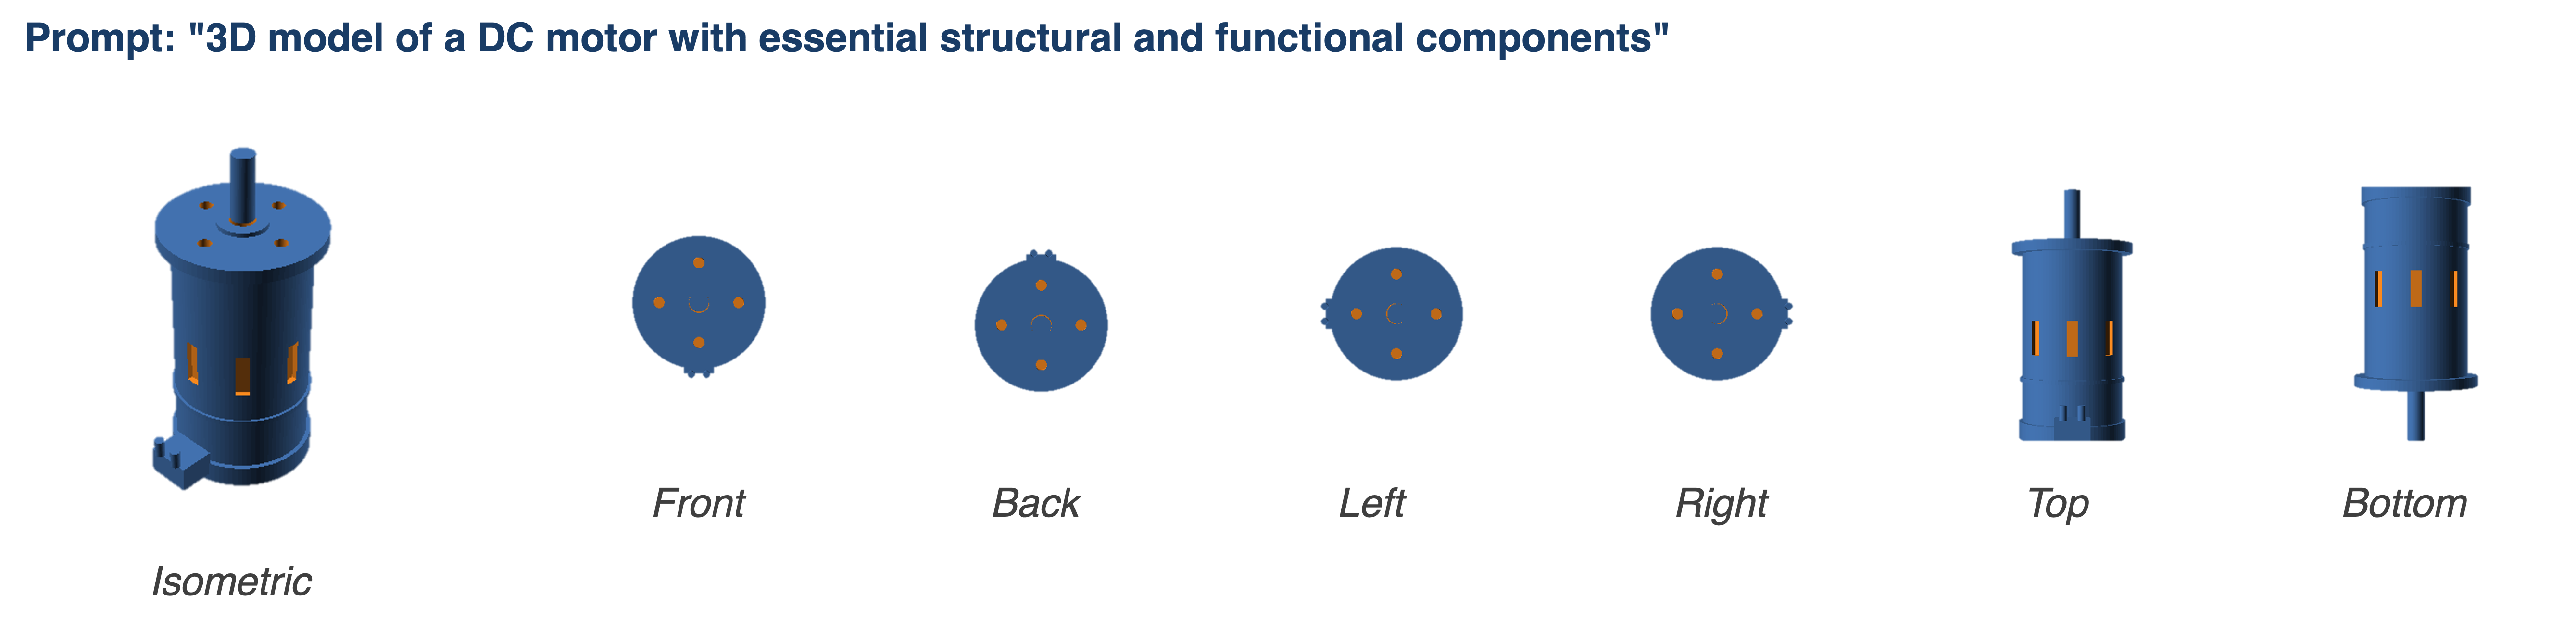
\includegraphics[width=0.8\textwidth]{figures/composites/Dc_motor.png}
    \caption{Multi-view rendering outputs from CRAFT. Each row shows a generated model from a text prompt: the isometric output alongside six orthographic views used for VLM assessment. This spatial coverage helps reveal geometric issues that may be hidden from a single viewpoint.}
    \label{fig:multiview-assessment}
\end{figure*}

\section{Additional Qualitative Examples}
\label{app:gallery}

To supplement the benchmark metrics, we include additional qualitative examples across simple, medium, and complex prompts. These examples illustrate both the diversity of generated outputs and the role of preserved parameters in enabling post-generation edits.

% \begin{figure*}[t]
% \centering
% \includegraphics[width=\textwidth]{figures/png/qualitative_comparison.png}
% \caption{Qualitative comparison across prompt complexity levels. Direct LLM generation baselines perform reasonably on simple primitives but degrade on functional objects and more complex assemblies. CRAFT maintains stronger quality across difficulty levels through its structured JSON intermediate representation and multi-view feedback, while CRAFT + retrieval further improves mechanical components by grounding generation in NopSCADlib specifications.}
% \label{fig:qualitative-comparison}
% \end{figure*}

% \begin{figure*}[t]
% \centering
% \includegraphics[width=\textwidth]{figures/png/cadence_gallery.png}
% \caption{Gallery of representative CRAFT outputs from the extended evaluation set. The examples span mechanical components, everyday objects, and abstract geometric forms, illustrating the breadth of the zero-shot parametric generation pipeline without task-specific fine-tuning.}
% \label{fig:extended-gallery}
% \end{figure*}

% \section{Public-System Case Study}
% \label{app:public-study}

% The public-system comparison in \secref{subSec:public-systems} is intended as a practical case study rather than a controlled benchmark. We include the full screenshots here for transparency because these systems target different representations and interaction styles.



\end{document}